\chapter{Análise Bibliográfica sobre simulação da disseminação de um vírus em redes relacionais, por Isaque Augusto da Silva Santos\label{chap:bibliometria:seraphritt}}

\section{Planejamento do estudo\label{ESS@seraphritt:questoes}}

No caso do meu trabalho, as perguntas que o nortearam foram:
\begin{itemize}
    \item Como são usadas as simulações de infecção viral? 
    \item Quais são as variáveis independentes e dependentes que tem sido usadas para o estudo do de infecções virais? 
    \item Qual a estrutura social da comunidade que pesquisa sobre o tema?
\end{itemize}

\subsection{O que já existe de pesquisa bibliométrica sobre esse tema?}

O tema da pesquisa está em voga atualmente devido a pandemia da Covid-19 e também, no contexto do Brasil, ao reaparecimento de doenças virais antes tidas como controladas ou até mesmo extintas, como por exemplo a Poliomielite \cite{mckeever_poliomielite_2022}. 

\cite{maheshwari_network_2020} fizeram uma pesquisa sobre o espalhamento da Covid-19 com distanciamento social, utilizando uma simulação multiagente.

Já \cite{wang_epidemic_2022} obtiveram resultados importantes nas suas simulações e que foram posteriormente comprovados em análises dos casos de Covid-19 na China, mostrando a eficácia de medidas como o isolamento social de casos confirmados.

\subsection{Uso do Bibliometrix e Biblioshiny}

Foram usadas a ferramenta e o \textit{workflow} proposto pelos autores do pacote Bibliometrix \cite{aria_bibliometrix_2017}.

\subsection{Limitações} O exercício relatado foi feito em três dias, envolvendo entre 3 e 4 horas de trabalho por dia, no período da noite.

\section{Coleta de dados\label{ESS@seraphritt:coleta}}

A coleta de dados feita usando o WoS (Web of Science) no dia 05 de Dezembro de 2022, acessado por meio do Portal de Periódicos da CAPES.

Foram feitas buscas em todas as coleções da WoS \textbf{Science  Citation  Index  Expanded (SCI-EXPANDED)}, \textbf{Social  Sciences  Citation  Index (SSCI)}, \textbf{Emerging Sources Citation Index (ESCI)}, \textbf{Arts \& Humanities Citation Index (A\&HI)}, \textbf{Conference Proceedings Citation Index - Science (CPCI-S)}, e \textbf{Index Chemicus(IC)}. Todavia, a maior parte dos artigos, cerca de 3479, encontram-se na coleção \textbf{SCI-EXPANDED}.

\subsection{Query de Busca}

Foi usada a \query\  de busca ilustrada nas linhas 1 a 9 da listagem \ref{query20221205-ser}.

\lstinputlisting[numbers=left,basicstyle=\normalsize\ttfamily,caption={\query\  de busca sobre simulação multiagente de disseminação viral em uma rede de convivência.},label=query20221205-ser]
{exploratory-data-analysis/seraphritt/PesqBibliogr/Virus-Network/query.txt}

Pode-se observar da linha 1 a linha 5 os sinais de `` () ``, `` * `` e a palavra `` or ``.  Os parenteses significam agrupamento, o asterisco significa qualquer letra ou símbolo ou nenhuma letra ou símbolo e a palavra \or\ significa a operação booleana `` ou ``.

Foi utilizado apenas um intervalo de 4 anos de publicação com o intuito de obter apenas os resultados mais recentes. Tendo em vista o grande número de artigos, essa faixa de somente 4 anos já obteve uma quantidade satisfatória de resultados que foram filtrados para serem somente do tipo \textbf{artigo}.

\subsection{Registros recuperados}

Doravante o dataset recuperado será chamado de ESS@seraphritt, que representa o acrônimo Epidemic Spreading and Simulation feito por Isaque Augusto da Silva Santos.

As informações gerais sobre o dataset ESS@seraphritt estão sumarizadas na tabela \ref{tab:ESS@seraphritt:Main}.

\begin{table}[htp]
\centering
\csvautotabular[separator=comma
%,filter not strcmp={\csvcolii}{}
]{exploratory-data-analysis/seraphritt/PesqBibliogr/Virus-Network/wos20220612_main_info.csv}
    \caption{Principais dados descritivos do \dataset\ ESS@seraphritt.}
    \label{tab:ESS@seraphritt:Main}
\end{table}

\section{Visualização de dados}

Esse gráfico \ref{ESS@seraphritt-cumulate} mostra a relação entre as fontes e as ocorrências acumuladas dos artigos durante o período de 4 anos (2018 a 2022).

\begin{figure}
    \centering
    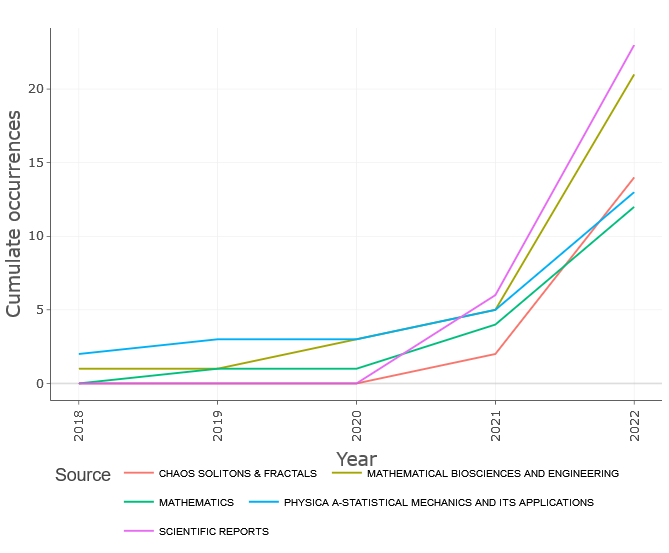
\includegraphics[width=\textwidth]{exploratory-data-analysis/seraphritt/PesqBibliogr/Virus-Network/souce_dynamics.png}
    \caption{Dinâmica das fontes no dataset ESS@seraphritt.}
    \label{ESS@seraphritt-cumulate}
\end{figure}

O mapa \ref{ESS@seraphritt-themap} a seguir possui a relação do desenvolvimento e a relevância dos temas presentes no dataset.

\begin{figure}
    \centering
    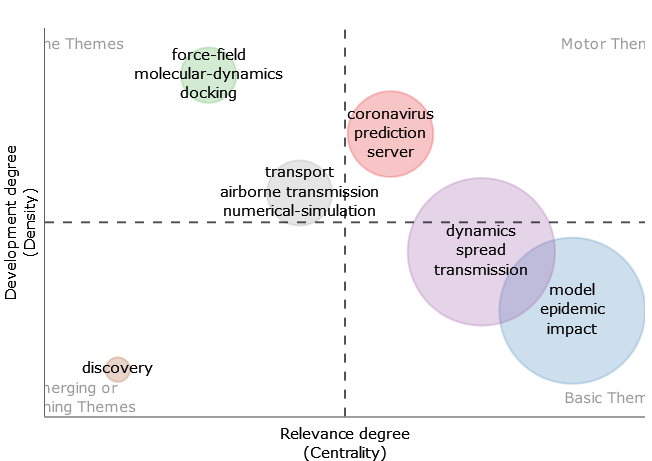
\includegraphics[width=\textwidth]{exploratory-data-analysis/seraphritt/PesqBibliogr/Virus-Network/themap.png}
    \caption{Mapa temático do dataset ESS@seraphritt.}
    \label{ESS@seraphritt-themap}
\end{figure}

A tabela \ref{tab:ESS@seraphritt:top10words} a seguir mostra as 10 palavras mais encontradas nos artigos e seu respectivo grupo.

\begin{table}[htp]
\centering
\csvautotabular[separator=comma
%,filter not strcmp={\csvcolii}{}
]{exploratory-data-analysis/seraphritt/PesqBibliogr/Virus-Network/CoWord_Factorial_Analysis_Words_By_Cluster.csv}
    \caption{Agrupamento de palavras do \dataset\ ESS@seraphritt.}
    \label{tab:ESS@seraphritt:top10words}
\end{table}

O grafo \ref{ESS@seraphritt-cocite} a seguir mostra a relação de citação entre os principais autores dos artigos presentes no dataset.

\begin{figure}
    \centering
    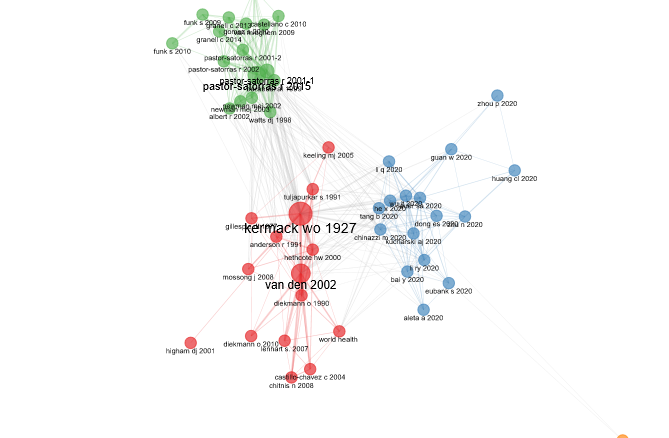
\includegraphics[width=\textwidth]{exploratory-data-analysis/seraphritt/PesqBibliogr/Virus-Network/cocitation.png}
    \caption{Rede de citação do dataset ESS@seraphritt.}
    \label{ESS@seraphritt-cocite}
\end{figure}

O gráfico \ref{ESS@seraphritt-collab} a seguir representa a relação entre os principais autores dos artigos presentes no dataset.

\begin{figure}
    \centering
    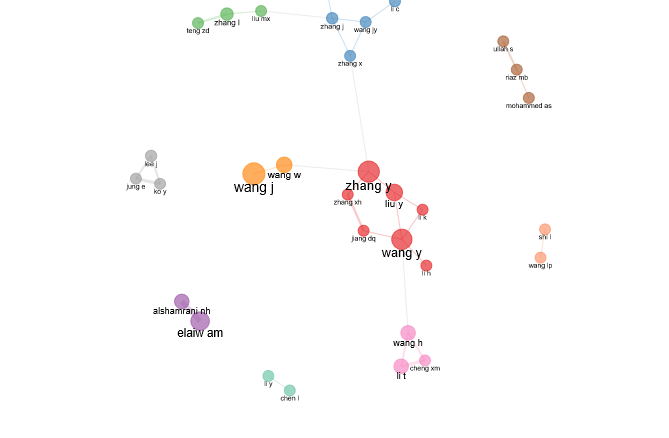
\includegraphics[width=\textwidth]{exploratory-data-analysis/seraphritt/PesqBibliogr/Virus-Network/collaboration.png}
    \caption{Rede de colaboração do dataset ESS@seraphritt.}
    \label{ESS@seraphritt-collab}
\end{figure}

O mapa \ref{ESS@seraphritt-world} evidencia a colaboração de cada país para a produção dos artigos presentes no dataset.

\begin{figure}
    \centering
    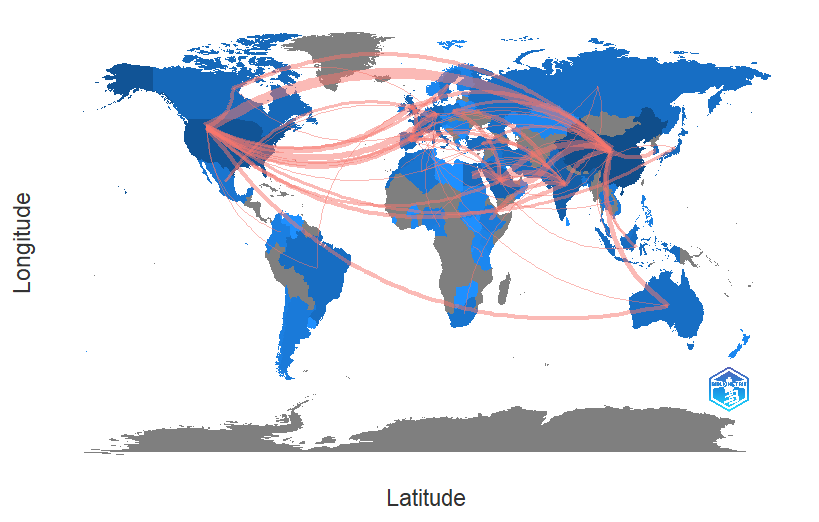
\includegraphics[width=\textwidth]{exploratory-data-analysis/seraphritt/PesqBibliogr/Virus-Network/world.png}
    \caption{Colaboração mundial do dataset ESS@seraphritt.}
    \label{ESS@seraphritt-world}
\end{figure}

A taxa de crescimento anual do dataset foi de 133.73 \%, e o gráfico da figura \ref{ESS@seraphritt-Crescimento} ilustra o crescimento da publicação entre 2018 e 2022. ``Isto posto, é possível concluir que o tema é bastante explorado atualmente, devido ao crescimento positivo observado.``

\begin{figure}
    \centering
    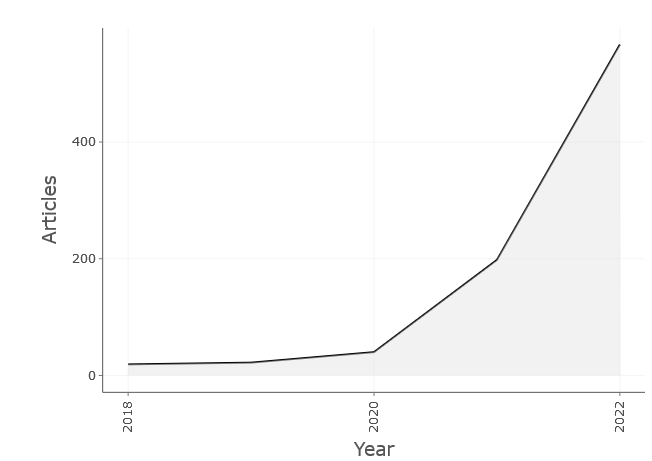
\includegraphics[width=\textwidth]{exploratory-data-analysis/seraphritt/PesqBibliogr/Virus-Network/newplot.png}
    \caption{Evolução de publicações no dataset ESS@seraphritt.}
    \label{ESS@seraphritt-Crescimento}
\end{figure}

\section{Interpretação}

As simulações de infecção viral são utilizadas para prever o surgimento de novas ondas, escolher a melhor estratégia para a contenção de contágio e minimizar os impactos na economia , vide \cite{maheshwari_network_2020-1}.  Existem vários tipos de modelos de simulação, o objetivo principal é descobrir o modelo que mais se aproxima da realidade e que seja mais eficiente.

As variáveis dependentes e independentes utilizadas para esse tipo de estudo variam de acordo com a doença que está sendo analisada, por exemplo nos casos da dengue, causada pelo vírus transmitido pelo mosquito \textit{Aedes aegypti}, uma variável independente importante pode ser o agente causador modificado ou não \ref{malik_modeling_2021}. 

No entanto, existem variáveis independentes gerais, como a taxa de transmissão, o tamanho da população, a taxa de mortalidade, probabilidade de deslocamento, entre outras. No que tange às variáveis dependentes, pode-se ter como exemplo o número de mortes, de saudáveis, infectados e imunes, como pode ser visto na simulação \ref{pudi_viral_nodate}.

A estrutura social dos pesquisadores é bem ampla e generalista, tendo em vista que o problema das infecções virais está presente em todo o mundo. Nesse ínterim, pode-se notar a variedade de nacionalidade dos autores dos artigos a seguir: \ref{zaplotnik_simulation_2020}, \ref{aranda_mathematical_2019},\ref{paul_mathematical_2018}.